
\subsection{Par compuesto (Sziklai)}

El par compuesto, Pseudo-Darlington, o Sziklai, por su inventor, se trata de una estructura formada por dos transistores conectados en cascada, similar al Darlington, pero que se diferencia de este en varios aspectos, para empezar se encuentra compuestos por la combinación de transistores \textit{PNP-NPN} o \textit{NPN-PNP}, es fácil observar que el par se comporta como el tipo de transistor que está en la entrada. El principal motivo del uso de esta estructura, se debió a la falta de transistores \textit{PNP} de buena calidad, en el pasado no había transistores realmente complementarios, con lo que se solía usar el par en la etapa de salida de amplificadores de potencia para reemplazar un transistor \textit{PNP} de potencia, mientras que en la otra rama se usaba un transistor \textit{NPN} o un Darlington. Otra diferencia con el Darlington, es que la tensión de encendido corresponde a solo una caída $V_{be}$, y no a dos como en el Darlington.\\
En caso de conectarse en forma directa los dos transistores, la ganancia de corriente del par compuesto es $\beta_{ef} = \beta_{1} \cdot \beta_{2} + \beta_{1}$, de orden similar pero algo menor que la del Darlington que es $\beta_{ef} = \beta_{1} \cdot \beta_{2} + \beta_{1} + \beta_{2}$. El agregado de una resistencia $R$ en el colector del primer transistor y base del segundo, tiene el efecto de reducir el $\beta$ efectivo, ya que se tiene:


\begin{equation}
\begin{rcases*}v_{be_{2}} = i_{c_{1}} \cdot (r_{\pi_{2}} // R) \\ i_{c_{2}} = gm_{2} \cdot v_{be_{2}} \\ \beta_{1} = \frac{i_{c_{1}}}{i_{b_{1}}}\end{rcases*} \Longrightarrow 
\end{equation}
 

\begin{equation}
i_{c_{2}} = gm_{2} \cdot i_{c_{1}} \cdot \frac{r_{\pi_{2}} \cdot R}{r_{\pi_{2} }+ R} = gm_{2} \cdot i_{c_{1}} \cdot \frac{ \frac{\beta_{2}}{gm_{2}} \cdot R}{r_{\pi_{2} }+ R} =
i_{c_{1}} \cdot \beta_{2} \cdot \frac{R}{r_{\pi_{2} }+ R} \Longrightarrow \\
\end{equation}
 

\begin{equation}
\frac{i_{c_{2}}}{i_{c_{1}}} =\frac{i_{c_{2}}}{i_{b_{1}} \cdot  \beta_{1} }= \beta_{2} \cdot \frac{R}{r_{\pi_{2} }+ R}  \Longrightarrow \\
\end{equation}


\begin{equation}
\boxed{\beta_{ef} = \frac{i_{c_{2}}}{i_{b_{1}}} = \beta_{1} \cdot \beta_{2} \cdot \frac{R}{r_{\pi_{2} }+ R}}
\end{equation}


El $\beta_{ef}$ aunque aún grande se ve disminuido por el agregado de $R$, la cual reduce la resistencia en el nodo de la base del segundo transistor, disminuyendo su tiempo asociado y mejorando el ancho de banda.\\

Para ver que el circuito está realimentado negativamente, hacemos un análisis incremental, si $I_{C_{1}}$ aumentara, aumentaría $V_{be_{2}}$, luego aumentaría $I_{C_{2}}$, con el consiguiente aumento de la caída en el resistor que estuviese conectado al emisor, por lo tanto aumentaría $V_{e_{1}}$, lo cual disminuye $V_{be_{1}}$ y finalmente esto disminuiría $I_{C_{1}}$, oponiéndose al aumento inicial, con lo cual se ve que está realimentado negativamente, haciendo un circuito mas estable comparándolo con un Darlington. \\
Lo fundamental es que por $R_{L}$ ahora pasa $I_{C_{1}}$ e $I_{C_{2}}$ con lo cual la ganancia a lazo abierto aumenta y esto mejora mucho el par conectado como seguidor.


\subsubsection{Análisis de pequeña señal por realimentación para el par compuesto como seguidor}


\begin{figure}[H] %htb
\begin{center}
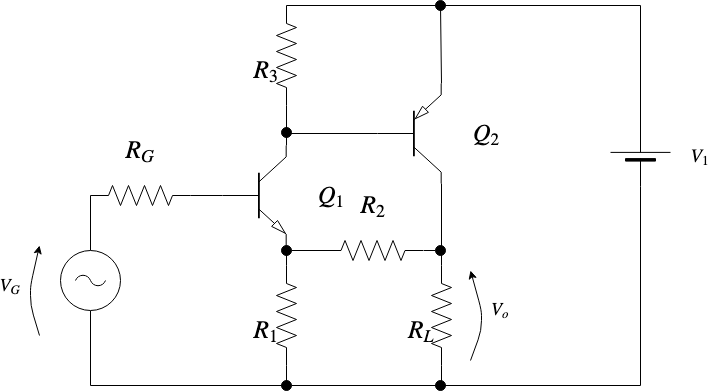
\includegraphics[width=0.9 \textwidth, angle=0]{./img/sziklai/sziklai1.png}
\caption{\label{fig:fig_sziklai_cir_1}\footnotesize{Par compuesto como seguidor}}
\end{center}
\end{figure}

El tipo de realimentación para la señal es la misma que con un único transistor en configuración seguidor, se muestrea tensión y se suma tensión, es un realimentador \textbf{serie-paralelo}

\textcolor{red}{\textbf{COMPLETAR!!}}


\clearpage